\newcommand{\resource}{{\sf resource}}
\newcommand{\resources}{{\sf resources}}
\newcommand{\Resource}{{\sf Resource}}
\newcommand{\Resources}{{\sf Resources}}

\section{Resources}

\index[subject]{resources|(}

\subsection{What Is A Resource?}

\index[subject]{resources!definition}

Perhaps the most fundamental concept in Vertebra is that of a \resource\nomenclature{resource}{Vertebra's fundamental unit of addressing}.  Conceptually, \resources{} are the fundamental unit of \textbf{addressing} in Vertebra.  In the abstract, a \resource{} represents something that matters to your application.  It might be a certain piece of data, a certain point of control, or a certain type of behavior.  Vertebra doesn't give it any meaning, your application does.

\index[subject]{resources!hierarchy}Just like concepts in your application, \resources{} can have relationships to each other.  In order to keep things relatively manageable, Vertebra's understanding of relationships is limited to a strict hierarchy.  In object-oriented parlance, it is the {\bf is-a} relationship embodied by a single inheritance model.  More formally, this means that any \agent{} that can be identified by a certain \resource, should also be identified by any ancestors of that \resource{}.

Given this framework, a rich variety of concepts should be representable.  A simple example of a set of resources are given in table \ref{tbl:res-philosopher}.  A visualization of the hierarchy they produce is given in figure \ref{fig:res-example2}.  Note the many dissimilar concepts are represented in this \resource{} hierarchy:

\begin{itemize}
	\item Citizenship
	\item Geography
	\item Professional Trades
	\item Language Fluency
\end{itemize}

In the example, we have used a path notation which lists all of the ancestor \resources{}, prepended to the \resource{} directly offered.  So the the entry ``{\sf/speaker/greek}'' indicates that Socrates speaks greek, which also implies that he speaks at all.

\begin{table}
	\begin{center}
		\begin{tabular}{| c | l |}
			\hline
			  Philosopher & Resources \\
			\hline
			\hline
			  \multirow{5}{*}{Socrates}              & /citizen/greece/athens \\
			                                         & /philosophy/classical\_greek \\
			                                         & /service/philosopher \\
			                                         & /service/stonemasonry \\
			                                         & /speaker/greek \\
			\hline
			  \multirow{5}{*}{Aristotle}             & /citizen/greece/athens \\
			                                         & /philosophy/aristotelianism \\
			                                         & /philosophy/peripatetic \\
			                                         & /service/philosopher \\
			                                         & /speaker/greek \\
			\hline
			  \multirow{9}{*}{Cicero}                & /citizen/rome \\
			                                         & /philosophy/stoic \\
			                                         & /service/lawyer \\
			                                         & /service/orator \\
			                                         & /service/philosopher \\
			                                         & /service/political\_theorist \\
			                                         & /service/statesman \\
			                                         & /speaker/greek \\
			                                         & /speaker/latin \\
			\hline
			  \multirow{8}{*}{Thomas Aquinas}        & /citizen/sicily \\
			                                         & /philosophy/scholasticism \\
			                                         & /service/political\_advisor \\
			                                         & /service/philosopher \\
			                                         & /service/lecturer \\
			                                         & /service/theologian \\
			                                         & /service/latin \\
			                                         & /speaker/italian \\
			\hline
			  \multirow{4}{*}{Nietzsche}             & /citizen/prussia \\
			                                         & /philosophy/weimar\_classicism \\
			                                         & /service/philosopher \\
			                                         & /speaker/german \\
			\hline
		\end{tabular}
	\end{center}
	\caption{Resources Possibly Offered By Various Famous Philosophers}
	\label{tbl:res-philosopher}
\end{table}

\begin{figure}
	\begin{center}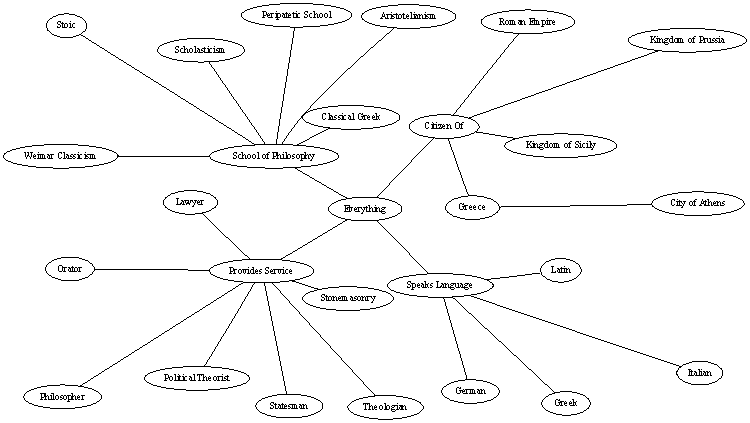
\includegraphics[width=\myfigwidth,height=\myfigheight,keepaspectratio]{figs/dot/res_example2}\end{center}
	\caption{Visualization of the Resource Hierarchy}\label{fig:res-example2}
\end{figure}

\subsection{Resources Are Groups Of Agents}

Hopefully it is evident from the above discussion that \resources{} are never actually realized \emph{per se}.  There is never a specific data structure or thing that can be said to be a \resource.  Instead, a \resource{} is more like a description or a tag.  What is significant about it is the set of things that it identifies.

Consequently, it's very useful to think of resources as sets of \agents{}.  \Agents{} that have something you want!  That's convenient, because it is very easy to use common techniques to visualize groups of \agents{} and their relationships.  An example using a Venn Diagram is shown in figure \ref{fig:res-example1}.

\begin{figure}
	\begin{center}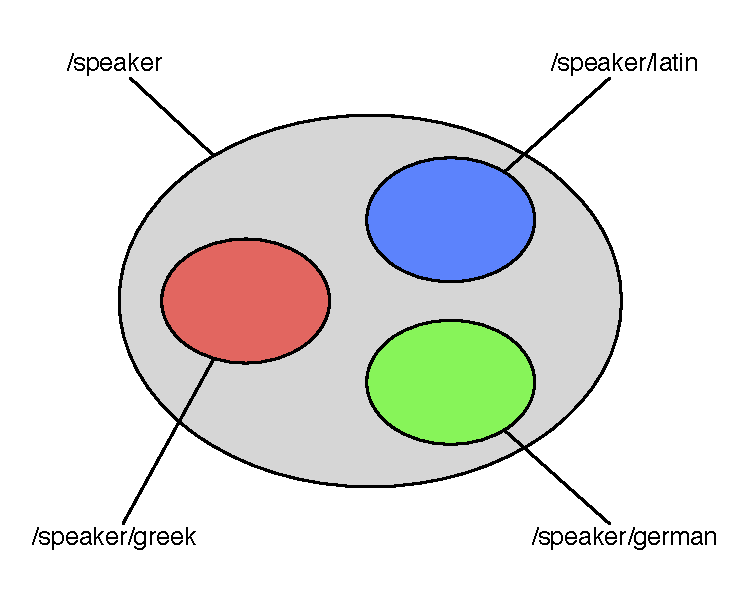
\includegraphics[width=\myfigwidth,height=\myfigheight,keepaspectratio]{figs/omnigraffle/res_example1}\end{center}
	\caption{Venn Diagram of a Resource Hierarchy}\label{fig:res-example1}
\end{figure}

\subsection{Resource Advertisement}

\index[subject]{advertising|see{resources}}
\index[subject]{resources!advertising|(}

In the more concrete sense, an \actor{} is said to ``provide'' a \resource{}.  When an \actor{} ``provides'' a \resource{} it causes any \agent{} that is configured with that \actor{} to ``advertise'' the same \resource{} (or perhaps an ancestor of it).  This causes requests to operate on that \resource{} to be directed to that \agent{}, which subsequently directs it to the appropriate \actor{}.

TODO: Put a bank example here.

\subsection{The Root Resource}

There is one final bit of errata.  It may not be so obvious from the above example, but all resources descend from a common, catch-all ancestor---the {\sf root} resource.  In our path notation, it is identified by the path ``{\sf /}''.

The root resource is rarely advertised on its own, but can be very useful when \resources{} are used for security and discovery purposes.

\subsection{The Advertising Process}

You may have noticed that I brushed over the details of ``advertising''.  Unfortunately we don't have all of the basics necessary to discuss advertising.  What I can tell you is that the \agent{} sends a message to the Vertebra security agent listing which \resources{} are offered.  We'll cover some more of the specifics in \ref{ref:direct-ops}.

\index[subject]{resources!advertising|)}

\index[subject]{resources|)}
